\documentclass[11pt]{article}
\usepackage[margin=1.1in]{geometry}
\usepackage{amsmath,amssymb}
\usepackage{booktabs}
\usepackage{graphicx}
\usepackage[hidelinks]{hyperref}
\usepackage{microtype}

% DRAFT 2026-09-29. Every number is regenerable by paper/paper_numbers.py and
% the census JSONs in paper/runs/; see the Reproducibility section. Items marked
% [TODO] must be resolved before release.

\title{Triangular FX Residuals on a Retail Feed Are Real,\\
Measurable, and a Fourteenth of Their Cost\\[6pt]
\large A preregistered census, a rejected thin-cross hypothesis, and
three unforced choices that together turned the negative into a positive}
\author{Michael M.\ Ross\\
\textit{Independent Researcher}\\
\small \texttt{michaelmross@cantab.net}}

\begin{document}
\maketitle

\begin{abstract}
\noindent
We measure triangular deviations on a retail foreign-exchange feed
(OANDA's v20 practice stream) under a protocol whose hypotheses, decision
gate, and synchronization tolerance were fixed before the data were
collected. Over ten London--New York sessions of EUR/USD, GBP/USD and
EUR/GBP (1.18 million ticks, 103{,}650 synchronized observations at
$\tau = 250$\,ms) there is no moment at which the three legs could be
traded at their quoted prices for a profit: the best executable cycle
observed is $-0.77$\,bp. The residual between the quoted cross and the
cross implied by the majors is real---a $+0.07$\,pip wedge with
$\sigma = 0.093$\,pip after removing its drifting level, reverting with
a half-life near five seconds---but one standard deviation of it is
7.2\% of the cost of a round trip in the cross, about one-fourteenth,
and less on the thin crosses. Every 30-second reversion bin loses between 1.1 and 1.6 pip
per trade at the spread quoted at the time. A preregistered follow-up
tested whether thinner crosses are priced more independently, requiring
the ratio $k$ of round-trip cost to residual $\sigma$ to fall below
EUR/GBP's $13.7$. It did not: AUD/NZD reads $k = 14.7$ and EUR/CZK
$17.3$ on the residual the signal trades, with zero executable cycles
in 155{,}110 further synchronized observations. Thinner crosses charge
more than their extra inefficiency is worth.

The negative result is expected, and consistent with interdealer
evidence that triangular opportunities were competed away by the late
2000s. What we report in full is how nearly it was not reported. The
decision gate, as first computed, returned PASS. That verdict needed
three choices, none fixed by the protocol and each reasonable in
isolation: judging reversion against the median spread rather than the
spread quoted at the time, which lets news-time dislocations clear the
bar while losing $1.3$\,pip per trade; measuring $\sigma$ on the raw
residual, whose between-hour level drift grows with sample length; and
pooling a calibration session declared throwaway in advance, which
lifted raw $\sigma$ across the gate's threshold. The second choice
alone would also have reversed the thin-cross test, passing both
arms. A fourth hazard, ordering ticks on a monotonic clock that
restarts at reboot, corrupted rate statistics fifteen-fold while
leaving the census count within 0.4\%. This note is a companion to a
daily-frequency ETF pairs study \cite{ross2026} and reaches the same
structural verdict at tick frequency.
\end{abstract}

\medskip
\noindent\textbf{Keywords:} triangular arbitrage; foreign exchange;
preregistration; market microstructure; transaction costs;
asynchronous sampling; negative result.

\smallskip
\noindent\textbf{JEL:} C58, F31, G14.

\section{Introduction}

Triangular arbitrage is the oldest no-arbitrage identity in foreign
exchange: the EUR/GBP rate must equal the ratio of EUR/USD to GBP/USD, up
to transaction costs. Deviations were documented at tick frequency in
the early 2000s \cite{aiba2002}, found to be short-lived and small on
high-frequency executable prices \cite{fenn2009}, shown to carry execution
risk that limits their exploitation even when they appear
\cite{kozhan2012}, and shown to have declined sharply once algorithmic
traders were admitted directly to the main interdealer platform
\cite{chaboud2014,ito2020}. Foucault, Kozhan and Tham \cite{foucault2017}
explain why the survivors are toxic to the liquidity providers who
quote them. Akram, Rime and Sarno \cite{akram2008} find the analogous
covered-parity deviations short-lived but economically significant in
size. None of this literature observes the question from where most
people who ask it sit: a retail feed, a retail account, retail latency.

That question has an obvious answer and a large file drawer. A retail
trader who measures a triangle, finds no opportunity, and stops, has
no reason to write it down; one who finds an apparent opportunity has
every reason not to. This note writes down the first case, and
concentrates on the second, because in the course of producing an
honest negative our own analysis produced a positive verdict that was
an artifact of three unforced choices. Each route is
generic to retail statistical-arbitrage measurement on a streamed feed,
and each produces output that looks clean.

The design follows the discipline of the companion ETF study
\cite{ross2026}: hypotheses and gate stated before data collection
\cite{nosek2018}, every component validated on synthetic ground truth
before touching live prices, and every correction made on the record
rather than silently. Section~\ref{sec:design} states the protocol and
Section~\ref{sec:feed} characterizes the feed. Section~\ref{sec:results}
gives the census verdicts. Section~\ref{sec:traps} dissects the three
choices and a clock hazard. Section~\ref{sec:interp}
relates the result to the ETF study.

\section{Design}\label{sec:design}

\subsection{Venue, triangles, and collection}

Prices are OANDA v20 streaming quotes on a practice account: best bid
and ask per instrument, each stamped by the venue, with the local
receive time recorded on both a monotonic clock and an NTP-disciplined
wall clock. The primary triangle is EUR/USD ($A$), GBP/USD ($B$) and
EUR/GBP ($C$), with $C = A/B$. Two further triangles were added for the
thin-cross test (Section~\ref{sec:prereg}): AUD/USD, NZD/USD and AUD/NZD,
whose legs both carry Asia-Pacific flow; and EUR/USD, USD/CZK and
EUR/CZK, a cross with genuine onshore price discovery in Prague. The
venue quotes USD/CZK rather than CZK/USD, so that leg is inverted on
ingest, which requires swapping as well as reciprocating the quotes
($\text{bid}' = 1/\text{ask}$, $\text{ask}' = 1/\text{bid}$). Getting
the swap wrong inverts the spread and makes every cycle look profitable
by exactly the round trip; the inverted triangle reproduces a
non-inverted one on synthetic data to machine precision on every
reported field. Each triangle streamed on its own account so that one
stream could not disturb another.

Collection ran 03:00--17:00 New York time on weekdays, covering the
London open through the New York close. The EUR/GBP census window was
declared in advance as the ten sessions 31 August--11 September 2026;
the thin-cross arms ran the ten sessions 14--25 September. Ticks were
written append-only to Parquet, with every reconnect and stream gap
logged. Collection was unattended and self-restarting. Recorded losses in the
03:00--17:00 window: ten minutes on 31 August (a late first start),
3.4 hours on 1 September (a collector failure), 3.2 hours on 3
September (the collector was terminated by a third-party software
installer), eight minutes on 9 September (a reboot), and 17 minutes in
both thin-cross arms on 24 September (an operating-system crash). Every
other session has at least 99.7\% coverage.

\subsection{Triangle algebra and the one-leg signal}

On mids, the log residual is
$\varepsilon_t = \ln A_t - \ln B_t - \ln C_t$. The deterministic cycle
returns at executable quotes are
\[
R_1 = \frac{C^{\text{bid}}_t\,B^{\text{bid}}_t}{A^{\text{ask}}_t} - 1,
\qquad
R_2 = \frac{A^{\text{bid}}_t}{B^{\text{ask}}_t\,C^{\text{ask}}_t} - 1,
\]
and a triangular arbitrage exists if and only if $R_1 > 0$ or
$R_2 > 0$, which requires $|\varepsilon_t|$ to exceed the sum of three
half-spreads. The statistical variant trades only the cross against the
rate implied by the majors, paying one spread rather than three. Its
signal is $z_t = (r_t - \mu_t)/\sigma_t$, where
$r_t = \ln C_t - \ln(A_t/B_t) = -\varepsilon_t$ and $\mu_t$, $\sigma_t$
are exponentially weighted moments with a 300-second half-life. A
position is entered on the cross against the sign of $z_t$ and closed
on reversion or after a timeout. Its round-trip cost is one full cross
spread.

Throughout, $k$ denotes the ratio of that round trip to the residual's
standard deviation, both in the cross's own pips. It is dimensionless,
and it is the entry threshold, in standard deviations, at which a
perfectly reverting residual would break even. Its reciprocal $1/k$ is
the residual's typical size as a fraction of what trading it costs:
EUR/GBP's $k = 14.0$ (Table~\ref{tab:census}) means one standard
deviation of the residual is one-fourteenth, or 7.2\%, of a round
trip, which is the figure in the title. ``Cost'' there means this
one-leg round trip, the cheaper way to trade the residual; the
three-leg cycle costs more (2.09\,bp against 1.51\,bp on EUR/GBP).
Residual $\sigma$ in
pips is not comparable across crosses: a EUR/GBP pip is 1.16\,bp, an
AUD/NZD pip 0.81\,bp and a EUR/CZK pip 0.041\,bp, so $\sigma$ alone
would make EUR/CZK's residual look thirty-four times EUR/GBP's when in
basis points it is only slightly larger. $k$ removes the unit.

\subsection{Synchronization and clocks}\label{sec:clocks}

The residual is only meaningful when all three quotes are current. An
observation is \emph{synchronized} if all three quote ages, measured on
the local monotonic clock, are below $\tau = 250$\,ms; sensitivity is
reported at $\tau \in \{100, 250, 500, 1000\}$\,ms. The value of $\tau$
was confirmed on a two-hour calibration session on 28 August by a
decision rule written down beforehand, and not revisited.

Three clocks are kept apart. Quote ages use the monotonic clock, which
cannot step. Cross-instrument ordering uses venue timestamps. Calendar
questions use the wall clock. Transport latency, the wall-clock receive
time minus the venue timestamp, is corrected per tick by reconstructing
the wall clock's error from NTP anchors taken at the start and end of
every run, including a rate term for the monotonic clock's own crystal
error, measured at $-0.7$ to $-1.6$\,ppm on this machine. None of this
affects the signal, which uses only quote ages; it matters for the
latency figures in Section~\ref{sec:feed} and, as Section~\ref{sec:reboot}
shows, for the ordering of ticks across runs.

\subsection{Preregistered hypotheses and gate}\label{sec:prereg}

The specification, written before any live data, states three
hypotheses and one gate:

\begin{itemize}\setlength{\itemsep}{2pt}
\item \textbf{H1 (deterministic census).} $P(R_1 > 0 \text{ or } R_2 > 0)
  \approx 0$ over synchronized executable quotes.
\item \textbf{H2 (residual structure).} Residual $\sigma$ at one-second
  sampling is at most 0.3\,pip.
\item \textbf{H3 (one-leg expectation).} Expected net per trade is
  negative at all thresholds under the measured cost model.
\item \textbf{Gate G1.} Proceed to paper trading only if $\sigma > 0.1$\,pip
  \emph{and} the conditional reversion curve shows expected capture
  within 30\,s exceeding 25\% of one EUR/GBP spread at some attainable
  entry level. Otherwise, report.
\end{itemize}

\noindent The specification also names the most likely outcome: that
the venue constructs the cross from the majors, leaving no independent
price to trade. The thin-cross prediction was written into both arms'
configuration files on 9 September, before either arm collected data:
\emph{the thin-cross hypothesis survives only if AUD/NZD's or EUR/CZK's
$k$ comes in below 13.7}, EUR/GBP's value on the sessions then
available. An earlier draft of the same prediction was phrased as
``$\sigma$ materially above EUR/GBP's'', which is ill-posed across
crosses for the reason given above; it was restated in $k$ before any
thin-cross data existed, and both configuration files record the
original wording. Section~\ref{sec:sigmabasis} records what the
registration did not fix.

\subsection{Ground-truth validation}

Before live data, the full pipeline---collector, replay, census, gate,
and paper-trading arm---was run end to end on two synthetic worlds with
known truth. In the \emph{derived} world the cross is $A/B$ plus a
spread, rounded to the venue's price grid; the pipeline must report
$\sigma$ at the rounding floor, no executable cycles, and a failing
gate. In the \emph{independent} world the cross carries an injected
Ornstein--Uhlenbeck deviation of 0.6\,pip with a four-second half-life;
the pipeline must recover both, find executable cycles, produce a
monotone reversion curve, and pass the gate. It does. The suite now
runs 65 checks, including the leg inversion, the lead--lag estimator's
sign on a known delay, and a replay of a synthetic day split into two
runs whose monotonic clocks overlap (Section~\ref{sec:reboot}). The
gate refuses to return a verdict on synthetic input, and the
paper-trading arm refuses to send an order without a passing gate and
unchanged frozen parameters.

\section{The feed}\label{sec:feed}

Table~\ref{tab:feed} summarizes what a retail trader sees. Three
features shape everything downstream.

\begin{table}[t]
\centering
\caption{Feed characteristics per triangle over its ten-session window.
Latency is local receive time minus venue timestamp, corrected per tick
for clock error. ``All three'' is the fraction of delivery bursts
carrying a quote for every leg. ``Venue spread $>$250\,ms'' is the
fraction of synchronized observations whose three venue timestamps span
more than 250\,ms.}
\label{tab:feed}
\begin{tabular}{lccc}
\toprule
 & EUR/GBP & AUD/NZD & EUR/CZK \\
\midrule
ticks & 1{,}181{,}278 & 1{,}103{,}896 & 995{,}713 \\
synchronized ($\tau=250$\,ms) & 103{,}650 (8.8\%) & 77{,}502 (7.0\%) & 77{,}608 (7.8\%) \\
synchronized hours & 132.9 & 139.5 & 139.5 \\
latency, median (ms) & 147--171 & 150--178 & 156--160 \\
delivery cadence (Hz) & 3.2 & 2.9 & 2.6 \\
bursts carrying all three legs & 12.2\% & 10.1\% & 11.6\% \\
cross ticks/min (legs) & 31 (48, 69) & 69 (31, 32) & 28 (50, 41) \\
venue spread $>$250\,ms & 13.7\% & 13.2\% & 10.9\% \\
\bottomrule
\end{tabular}
\end{table}

\emph{The stream is coalesced.} Quotes arrive in bursts about three
times a second, one to three instruments at a time, rather than tick by
tick. A synchronized observation is therefore possible only at the end
of a burst that happens to carry all three legs, one burst in eight
to ten. This bounds what the census can see: a deviation that opens and
closes inside one flush interval is invisible, and the interdealer
literature places cost-exceeding deviations well below a second
\cite{fenn2009,chaboud2014}. The census is a census of what a retail
trader can observe, which is the population that matters to the
retail question.

\emph{Receive-synchronized is not venue-synchronized.} Between 11 and
14\% of synchronized observations carry venue timestamps spanning more
than 250\,ms, because a local processing stall delivers quotes stamped
at different moments within a few milliseconds of each other. On
EUR/GBP the residual's standard deviation is the same with and without
these observations (0.098\,pip in both), so the contamination is
reported but not material here. It grows with machine load.

\emph{The cross is derived, plus a markup.} The specification's direct
test of internal derivation is the share of synchronized observations
with $|\varepsilon| < 0.05$\,pip. On EUR/GBP it is 31.8\%. The
residual's median is $+0.068$\,pip and it is positive in 78\% of
observations, which is the signature of a cross computed from the
majors with a persistent wedge, not a cross with no wedge. The
literal test calls such a cross ``not derived'' because the wedge
moves it away from zero, so the informative quantity is variance
around the wedge, not distance from zero. Decomposing that variance
by extrapolating $\sigma^2(\tau)$ to $\tau = 0$ attributes 8.5\% to the
venue's price grid, 6.4\% to cross-pair asynchrony, and at most 85\% to
anything that could be independent pricing of the cross; the last
figure is an upper bound because asynchrony survives at $\tau = 0$.

Lead--lag, which the specification needed to justify trading the cross
rather than a major, is not identified on this feed. The event study
around $|z| \ge 2$ crossings is confounded by flush order: one leg
supplies 94--99\% of synchronized observations in every triangle,
because the venue flushes it last, so ``which instrument closed the
dislocation'' recovers that base rate (lift over base rate 0.5--1.0).
The Hayashi--Yoshida estimator \cite{hayashi2005}, which needs no
common grid and is the standard remedy for asynchronous sampling
\cite{epps1979}, returns profiles flat to within 0.025 in correlation across
$\pm 2$\,s in all three triangles. Its argmax is reported by the pipeline and
carries no information; we draw no lead--lag conclusion. AUD/NZD
illustrates why tick counts are not a substitute: its cross is quoted
twice as often as either leg, the reverse of EUR/GBP, without leading
them in the only estimator that could say so.

One venue behaviour is worth recording because it is regular enough to
predict. AUD/NZD and NZD/USD fall silent from 14:59:05 to 15:04:55 New
York time (to within a second), a 350-second break, on eight of eight
Monday--Thursday sessions, including the session interrupted by the crash, and on
neither Friday. 15:00 in New York is 07:00 the next morning in New
Zealand, a business day except after a Friday. We have not established
the mechanism; stale quotes are excluded by the synchronization rule,
so the break costs observations and contaminates nothing. New Zealand
daylight saving began on 27 September, after collection ended; the
break should move an hour earlier if the explanation is right, and we
record that prediction untested.

\section{Results}\label{sec:results}

\subsection{H1: there is nothing to take}

Table~\ref{tab:census} gives the census. Across 258{,}760 synchronized
observations in three triangles there is no executable cycle. The best
cycle ever observed is $-0.77$\,bp on EUR/GBP, $-2.87$\,bp on AUD/NZD
and $-1.48$\,bp on EUR/CZK, against median three-leg costs of 2.09,
4.37 and 3.13\,bp. H1 is confirmed in every triangle.

\begin{table}[t]
\centering
\caption{The census, each triangle over its declared ten-session
window. $\sigma$ is the demeaned residual (the residual net of the
signal's own running mean), in the cross's pips and in basis points.
$k$ is round trip over $\sigma$. ``Best bin, net'' is the
least-negative 30-second reversion bin with $n \ge 30$, charged half
the cross spread quoted at entry plus half at exit.}
\label{tab:census}
\begin{tabular}{lccc}
\toprule
 & EUR/GBP & AUD/NZD & EUR/CZK \\
\midrule
executable cycles $R_1>0$ or $R_2>0$ & 0 & 0 & 0 \\
best cycle observed (bp) & $-0.77$ & $-2.87$ & $-1.48$ \\
three-leg cost, median (bp) & 2.09 & 4.37 & 3.13 \\
cross round trip, median (pip / bp) & 1.30 / 1.51 & 3.40 / 2.74 & 54.0 / 2.22 \\
residual $\sigma$ (pip / bp) & 0.093 / 0.108 & 0.231 / 0.187 & 3.13 / 0.129 \\
$\sigma$ as a share of the round trip & 7.2\% & 6.8\% & 5.8\% \\
$k$ & 14.0 & 14.7 & 17.3 \\
best 30\,s bin, net of quoted spread (pip) & $-1.10$ & $-3.07$ & $-54.4$ \\
Gate G1 & FAIL & FAIL & FAIL \\
\bottomrule
\end{tabular}
\end{table}

\subsection{H2: a real residual, one-fourteenth of its cost}

Sampled on a one-second grid, the EUR/GBP residual has standard
deviation 0.087\,pip, well inside H2's bound of 0.3, with excess
kurtosis near 5 and an AR(1) half-life of 5.3\,s (4.2\,s at 100\,ms
sampling). H2 is confirmed. The residual is not zero, as the
specification feared it might be; it is a genuine, rapidly reverting
quantity, and it is small. Measured the way the census measures it,
over every synchronized observation and net of the drifting level the
signal removes, $\sigma$ is 0.093\,pip against a 1.30\,pip round trip:
7.2\%, or one-fourteenth ($k = 14.0$). The thin crosses come in at
about one-fifteenth (AUD/NZD, 6.8\%) and one-seventeenth (EUR/CZK,
5.8\%). H2's own measure differs in two respects---it samples on a
regular one-second grid, weighting each second rather than each
observation, and it does not remove the drifting level---and gives the
smaller 0.087\,pip. Sensitivity to $\tau$ is flat between 100
and 250\,ms (94{,}439 and 103{,}650 observations, $\sigma$ 0.098 and
0.098\,pip) and jumps at 500\,ms (318{,}352 observations, $\sigma$
0.133), exactly where a coalesced three-hertz feed starts admitting
quotes from different bursts.

\subsection{H3 and the gate}

The conditional reversion curve (Figure~\ref{fig:gate}) is the object
the specification uses to set thresholds without a backtest grid
search. Capture within 30 seconds rises monotonically in $|z|$, is
precisely estimated (Newey--West \cite{neweywest1987} intervals,
with the bin the gate rests on cross-checked by circular block
bootstrap \cite{kunsch1989}), and
never approaches the cost of taking it. Charged half the cross spread
quoted at entry and half at exit, every bin loses money; the best nets
$-1.10$\,pip on EUR/GBP. The specification's own threshold rule,
$k_{\text{in}} = \arg\max_x [\text{capture}(x) - \text{spread} -
2\cdot\text{slippage}]$, has no positive maximum at any $x$, even at
zero slippage. H3 is confirmed without a trade: no threshold exists at
which the paper-trading arm would have had positive expectation.

Gate G1 fails on the declared EUR/GBP window. Its $\sigma$ criterion
reads 0.0976\,pip against a bar of 0.10. Its capture criterion
\emph{passes}, on a single bin: $z \ge 5$, $n = 35$, capturing
0.92\,pip (95\% interval 0.74--1.10) against a bar of 0.325\,pip.
That bin loses 1.31\,pip per trade at the spread quoted at the time.
The gate also fails in both thin-cross arms, on its capture criterion.
No paper trading was run; the specification's fallback, a few days of
pipeline validation, was not needed to reach any conclusion and was
not run.

\subsection{The thin-cross hypothesis is rejected}\label{sec:thin}

\begin{table}[t]
\centering
\caption{$k$ (round trip over $\sigma$) on four bases for $\sigma$.
\emph{Raw} is the residual's sample standard deviation;
\emph{within-hour} pools variance within clock hours; \emph{demeaned}
is the residual net of the signal's running mean; \emph{spread-matched}
is the median over clock hours of that hour's own spread over that
hour's demeaned $\sigma$ (interquartile range in brackets). \emph{Drift}
is the share of raw variance that is between-hour drift of the
residual's level. The preregistered bar, $k < 13.7$, applies to the
thin crosses (EUR/GBP is the benchmark it came from); thin-cross values
below it are in bold.}
\label{tab:kbasis}
\begin{tabular}{lccccc}
\toprule
 & raw & within-hour & demeaned & spread-matched & drift \\
\midrule
EUR/GBP & 13.3 & 13.7 & 14.0 & 16.0 [14.7, 16.9] & 5.3\% \\
AUD/NZD & \textbf{13.4} & 14.5 & 14.7 & 16.9 [16.0, 17.7] & 15.4\% \\
EUR/CZK & \textbf{10.1} & 16.8 & 17.3 & 19.8 [18.0, 22.1] & 63.7\% \\
\bottomrule
\end{tabular}
\end{table}

Both thin crosses fail the preregistered test on the residual the
signal trades: AUD/NZD $k = 14.7$ and EUR/CZK $k = 17.3$, against a bar
of 13.7 (Table~\ref{tab:kbasis}). The verdict holds on the within-hour
and spread-matched bases and session by session: AUD/NZD falls below
13.7 on two of ten sessions (the FOMC day and a Friday whose last hour
quoted the cross at 12.9 pip), EUR/CZK on none (Figure~\ref{fig:kbasis}).
Neither arm produced an executable cycle, and the best reversion bins
net $-3.07$\,pip on AUD/NZD and $-54.4$\,pip on EUR/CZK. AUD/NZD's
margin over EUR/GBP is modest and their spread-matched interquartile
ranges overlap; EUR/CZK is clearly worse. The hypothesis predicted the
opposite ordering. In basis points the thin crosses' residuals are
1.2 (EUR/CZK) and 1.7 (AUD/NZD) times EUR/GBP's, while their round
trips are 1.5 and 1.8 times as wide.

On the raw basis, however, both arms pass. Section~\ref{sec:sigmabasis}
explains why that basis is not the one to trust, and records that the
registration did not say.

\section{Three routes to a false positive}\label{sec:traps}

The gate's PASS required three choices to align, and each is the kind
of choice a careful analyst makes without noticing it is a choice. The
first two concern what the residual is compared with; the third, what
the sample is. Individually, the first makes the gate's capture
criterion pass on any sample, and the second reverses the thin-cross
test; only together, with the third, did they pass the gate.

\subsection{The cost basis: median spread against quoted spread}
\label{sec:costbasis}

\begin{figure}[t]
\centering
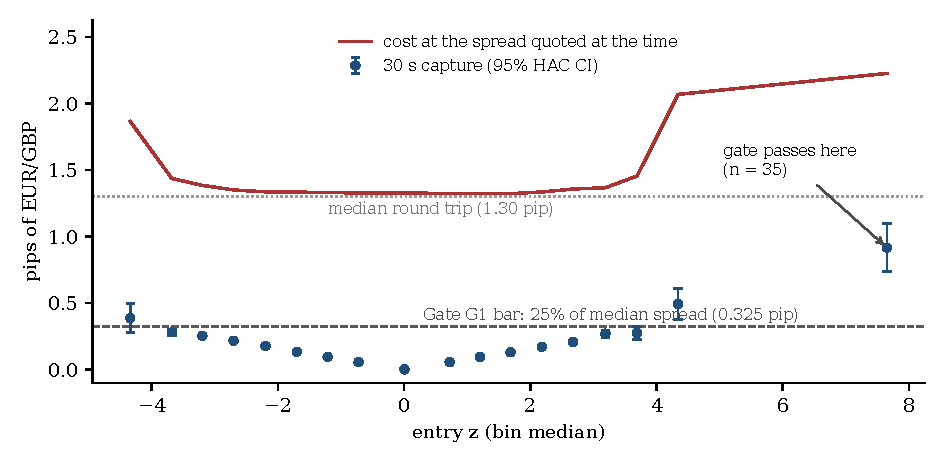
\includegraphics[width=.92\textwidth]{fig_gate.pdf}
\caption{EUR/GBP 30-second capture by entry $z$, declared window.
The gate's capture criterion compares capture with a quarter of the
\emph{median} spread (dashed); trading it costs the spread quoted
\emph{at the time} (red). The extreme bins clear the first and fall
furthest short of the second, because they occur when the cross is
quoted wide.}
\label{fig:gate}
\end{figure}

The gate's capture criterion is stated against ``one EUR/GBP spread'',
and the natural implementation divides by the median. The bin that
clears it is the one furthest from being tradeable. Of the 35
observations in the $z \ge 5$ bin, 83\% occur when the cross is quoted
wider than its median; the median spread at entry is 2.4\,pip against
1.3 overall. Two thirds fall within the conventional 08:30 and 10:00
New York release slots. They span nine sessions, so this is not one
event. The observations are not stale quotes either: their three legs
were a median 41\,ms apart at the venue, and the subset under 250\,ms
captures slightly more (0.96\,pip). Macroeconomic releases move
exchange rates within seconds \cite{andersen2003} and widen quoted
spreads \cite{mancini2013}, and the triangle's residual inherits both.
The residual genuinely dislocates on news, genuinely reverts within
30 seconds, and genuinely cannot be traded, because the spread widened
by more than the dislocation.

Figure~\ref{fig:hourly} shows the same mechanism across the whole
sample. The hours with the largest residual $\sigma$ are the hours with
the widest spread, so any statistic that takes $\sigma$ from the
volatile hours and cost from the typical hour overstates
tradeability. The repair is to charge each observation the spread
quoted when it occurred. The census now reports capture net of that
cost beside every reversion bin, so the two can no longer be read
apart.

\begin{figure}[t]
\centering
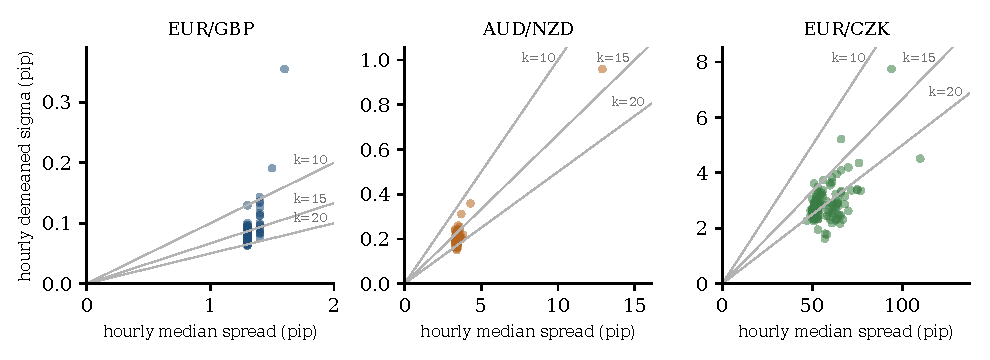
\includegraphics[width=.98\textwidth]{fig_hourly.pdf}
\caption{Hourly demeaned residual $\sigma$ against the hour's median
cross spread, one point per clock hour. Grey lines are constant $k$.
High-$\sigma$ hours are wide-spread hours in every triangle.}
\label{fig:hourly}
\end{figure}

\subsection{The \texorpdfstring{$\sigma$}{sigma} basis: level drift and an
unspecified estimator}\label{sec:sigmabasis}

The raw standard deviation of the residual includes the drift of its
level between hours and days, which no 30-second trade can capture and
which accumulates with sample length. Table~\ref{tab:kbasis} measures
it: between-hour drift is 5\% of EUR/GBP's raw variance, 15\% of
AUD/NZD's and 64\% of EUR/CZK's. For EUR/CZK the raw $\sigma$ over ten
sessions is 5.34\,pip while no single session exceeds 4.0, and raw $k$
falls to 10.1. On the raw basis both thin arms clear the preregistered
bar of 13.7 (Figure~\ref{fig:kbasis}, left). On every basis that
removes the drift, neither does.

\begin{figure}[t]
\centering
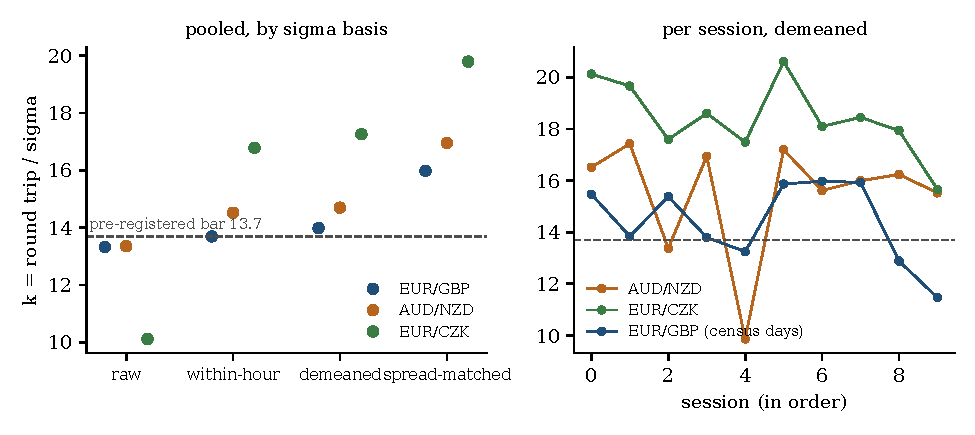
\includegraphics[width=.98\textwidth]{fig_kbasis.pdf}
\caption{Left: pooled $k$ per triangle on four $\sigma$ bases, against
the preregistered bar. Only the raw basis puts the thin crosses below
it. Right: per-session $k$ on the demeaned basis; the EUR/GBP series is
its census window, not the same dates.}
\label{fig:kbasis}
\end{figure}

The registration fixed the threshold but not the estimator behind it,
and we must record when the ambiguity was resolved. It was noticed on
16 September, after three thin-cross sessions, when AUD/NZD's raw $k$
of 12.5 would have been reported as beating 13.7. We adopted the
demeaned basis at that point. The argument for it does not depend on
the data: the signal preregistered in the configuration
($z_t = (r_t - \mu_t)/\sigma_t$, with $\mu_t$ an exponentially weighted
mean) trades the demeaned residual, so the demeaned $\sigma$ is the one
the strategy's breakeven depends on, and a raw $\sigma$ that grows with
sample length is not a property of the cross at all. The argument
against treating the choice as post hoc is that the within-hour and
spread-matched bases, which impose no model of the mean, reach the same
verdict. But a reader should know that on the only basis a naive
implementation would use, the preregistered test passes twice.

The structure being removed is the same one the companion study found
at daily frequency, where credible ETF spreads combined fast mean
reversion with a fractional wander of their level \cite{ross2026}. Here
the fast component reverts in seconds and the wander operates over
hours; in both cases a statistic that mixes the two describes neither.

\subsection{Sample composition: a declared throwaway, pooled}
\label{sec:pooling}

The census tooling analyses every collected session unless told
otherwise. The first full census run was not told otherwise, and it
included the Phase 0 calibration session of 28 August, which the
protocol had declared throwaway before it ran, along with test runs on
27 August. That session was the sample's high-$\sigma$
outlier. Pooled in, it raised raw $\sigma$ from 0.0976 to 0.124\,pip,
between-hour drift from 5\% to 39\% of raw variance, and the gate's
$\sigma$ criterion from fail to pass. With the capture criterion
already passing on the median-spread basis, Gate G1 returned PASS, and
it was reported internally as the preregistered verdict for more than
two weeks before the pooling was noticed while preparing this note.

It is worth tracing what the PASS required. On the demeaned basis the
pooled sample's $\sigma$ is 0.095\,pip, below the threshold, so the
PASS needed the raw basis and the pooling together, and then the
median-spread capture bar. Three choices, none specified by the
protocol and each individually reasonable, had to align, and they did,
by default. The pooled run's recorded verdict is retained in the
archive, labelled as the error it is.

\subsection{A clock that restarts at reboot}\label{sec:reboot}

The fourth hazard is mechanical, and it is included because it
corrupts statistics silently and because we reproduced it while
preparing this note. The replay engine originally ordered all ticks by
the monotonic receive clock, which is the right order within a process
and the only order the live engine ever sees. But the monotonic clock
restarts at every reboot, and after a mid-census reboot on 9 September
the runs of 1, 2, 3, 9, 10 and 11 September occupied overlapping
monotonic ranges (Figure~\ref{fig:reboot}). Over all twenty EUR/GBP
runs, a global sort interleaved them tick by tick: 37{,}979 changes of
run in the ordered sample, against 19 for the runs correctly laid end
to end.

\begin{figure}[t]
\centering
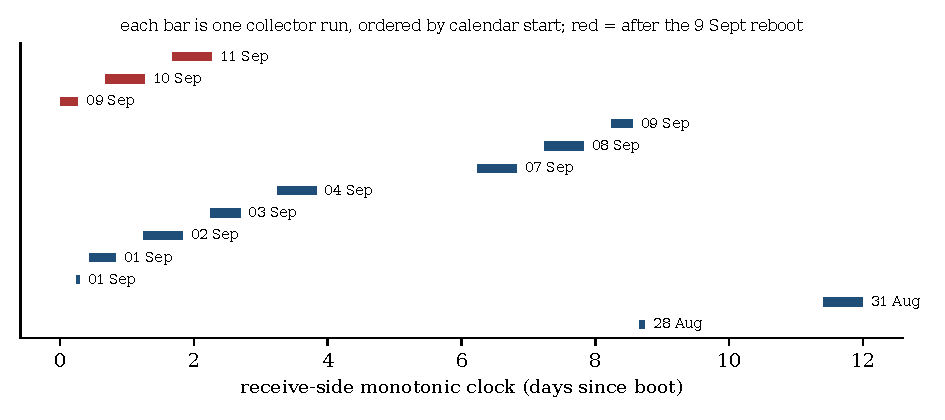
\includegraphics[width=.92\textwidth]{fig_reboot.pdf}
\caption{Monotonic-clock range of each EUR/GBP collector run, ordered
by calendar start. After the 9 September reboot the clock restarted
near zero, so later runs (red) overlap earlier ones and a sort on this
clock interleaves different days.}
\label{fig:reboot}
\end{figure}

The census count barely moved: over the same runs the interleaved
replay yields 108{,}596 synchronized observations against 109{,}028
correctly ordered, a loss of 0.4\%, because the replay resets its quote book at every change of
run. Rate and duration statistics were not so lucky. The tick rate on
9 September read 2.0, 3.1 and 4.7 per minute against true values of
30.1, 46.4 and 69.5, because the denominator included the machine's
uptime before the reboot; the census's ``observed hours'' spanned
overnight gaps; resampling carried the last value forward across them;
and any horizon statistic could pair ticks from different days. The
repair orders runs by wall-clock start and ticks within a run by the
monotonic clock, and gives every downstream time difference an axis on
which runs are separated by more than any horizon in use. A synthetic
day split into two runs with deliberately overlapping clocks now
reproduces the unsplit synchronized count exactly and its hours and
tick rates to within 0.1\%.

The script that generates this note's numbers repeated the error in
its first version, reporting a 14-day ``gap'' in the NZD stream on the
session interrupted by the crash. Any analysis that sorts a streamed
log on a process-local clock inherits it.

\subsection{What the routes share}

The three routes of Sections~\ref{sec:costbasis}--\ref{sec:pooling}
have a common form. A quantity the protocol names---``one spread'',
``$\sigma$'', ``the sample''---admits more than one estimator; the
default estimator mixes a component the strategy cannot trade with one
it can; and the mixing flatters the strategy. The median spread mixes
calm hours into the cost of news-time trades. The raw $\sigma$ mixes
level drift into the size of a reverting residual. The default sample
mixes a declared calibration session into the census. None produces a
visible anomaly, and each passes every check that looks only at its
own output. The general repair is to tie each quantity to the thing
actually traded---the spread paid, the residual the signal trades, the
sample the protocol declared---and to write that tie into the
registration, which ours did not do for any of the three.

\section{Interpretation}\label{sec:interp}

The retail triangle is closed. That was expected, and the census adds
a retail-feed measurement to the interdealer evidence rather than
contradicting it: any deviations that exceed three half-spreads must,
if they occur, open and close inside one flush interval of this feed,
where they are taken by participants
whose costs and latencies are orders of magnitude below a retail
account's \cite{chaboud2014,ito2020}. The statistical variant fails for
a different and more instructive reason. The residual is not an
artifact of rounding or asynchrony, which together explain perhaps
15\% of its variance, and it reverts quickly and reliably. It is simply
priced: at a fourteenth of the cross's spread on EUR/GBP and less on
the thin crosses, the venue quotes the cross wide enough that its own
deviation from parity is never worth trading against it.

The thin-cross result sharpens this. If thinner crosses were priced
more independently, their residuals should be larger relative to their
spreads. They are not. In basis points AUD/NZD's residual is somewhat
larger than EUR/GBP's and EUR/CZK's about the same, while their spreads
are 1.8 and 1.5 times wider. A venue that prices a thin cross
independently still sets its spread to cover the risk of that
independence, and the spread grows faster than the residual it
covers. We offer this as a description of three triangles on one
venue, not as a law.

The companion ETF study reached the same structural verdict at daily
frequency: detection real, return absent, and the gap filled by
exactly the width a liquidity provider would charge \cite{ross2026}.
Both studies also found their validation suites passing while the real
data had structure the synthetic generators lacked---a noise-dominated
spread there, a drifting wedge and news-time spreads here---and in both
the repair was a comparison calibrated to the data rather than to
convenience.

\section{Limitations}

\emph{Venue and account.} All data are from one venue's practice
stream. Practice prices are not guaranteed to equal live prices, and a
practice fill carries no queue, impact or last-look rejection; because
no trade was taken, only the first caveat applies, but it applies to
every number here. \emph{Resolution.} The stream is coalesced at about
three hertz and received with a median latency near 160\,ms, so the
census cannot see sub-second deviations and does not claim to.
\emph{Sample.} Ten sessions per triangle, three triangles, one month,
one collection window (03:00--17:00 New York), which excludes AUD/NZD's
Asian hours and EUR/CZK's early Prague morning. \emph{Protocol
deviations.} Three are reported in the text: the pooled census of
Section~\ref{sec:pooling}, the $\sigma$ basis adopted after three
thin-cross sessions (Section~\ref{sec:sigmabasis}), and the absence of
the paper-trading fallback, whose purpose was pipeline validation
rather than evidence. \emph{Events.} The event calendar used to flag
release windows was incomplete, missing several US releases that fall
inside the window; it enters no verdict, and Section~\ref{sec:costbasis}
classifies by clock time instead. \emph{Estimators.} The thin-cross
comparison rests on a single threshold computed from part of the
EUR/GBP sample; its value on the full census is 13.3 to 14.0 depending
on basis, which does not change either arm's verdict on the bases that
remove drift. The lead--lag analysis is uninformative on this feed and
no conclusion should be drawn from it. \emph{Machine.} Collection ran
on a single desktop, which rebooted three times during the study, once
by crashing; the
resulting losses are small and recorded, and the clock treatment is
described in Section~\ref{sec:clocks}.

\section{Conclusion}

On a retail FX feed, over thirty sessions and three triangles, there
is no triangular arbitrage and no statistical strategy on the cross's
residual that pays its own spread. The residual is real, measurable
and quickly reverting; it is also between a fourteenth and a
seventeenth of the cost of trading it, and thinner crosses make that
ratio worse rather than better. The preregistered hypotheses are
confirmed, the decision gate fails, and the thin-cross hypothesis is
rejected.

The finding we would most like a reader to take away is not the
negative, which the literature predicts, but the three ordinary
choices through which our own pipeline reported a positive: a median
where the spread paid belonged, a raw standard deviation where the
traded residual belonged, and a default sample where the declared one
belonged. Each is a single line of code and a sentence of
specification. A preregistration that fixes thresholds without fixing
the estimators they are compared with leaves the verdict to those
defaults, and ours nearly did.

\section*{Reproducibility}

The collector, replay engine, census, validation suite, and the
scripts behind every number and figure in this note are in
\texttt{fx\_statarb/} of the repository

\begin{center}
\url{https://github.com/michaelmross/stat-arb}\quad
\textbf{[TODO: push fx\_statarb/ and confirm path]}
\end{center}

\noindent archived under DOI \textbf{[TODO: Zenodo DOI]}.
\texttt{paper/paper\_numbers.py} regenerates \texttt{paper\_numbers.json}
from the tick logs and the census outputs in \texttt{paper/runs/},
which are produced by \texttt{phase1\_analyze.py} with the explicit
session lists given there; \texttt{paper/make\_figures.py} regenerates
all four figures. The pooled census of Section~\ref{sec:pooling} is
retained in \texttt{paper/runs/eurgbp\_all/}. \texttt{selftest.py}
runs the 65 ground-truth checks with no credentials and no network.

Price data are OANDA practice-account quotes retrieved under a personal
API token and are not redistributed. In their place the archive
carries \texttt{data\_manifest.json}: SHA-256, row count and run
identifiers for every Parquet part file behind the three census
windows (1{,}181{,}311, 1{,}103{,}896 and 995{,}713 rows; the EUR/GBP
file total exceeds the census by the 33 rows of a quarantined
duplicate run, excluded on the record). \textbf{[TODO: confirm OANDA's
terms on redistribution of practice-feed data.]}

\section*{Acknowledgments}

The collection and analysis pipeline was built and operated in agentic
sessions with Anthropic's Claude Opus 5, and this note was drafted by
Claude Fable 5.1 from the archived outputs. Several errors made within
that workflow are reported in the text: the pooled gate verdict, the
raw-basis $k$ comparison, an early overestimate of the reboot bug's
effect on the census count, and a reversed sign in the lead--lag
estimator's printed interpretation, which led to a claim about AUD/NZD
that the flat profiles do not support. Each was found by recomputation
against ground truth before this draft. Unlike the companion note, this
draft has not yet been verified by an independent session.
\textbf{[TODO: independent verification pass.]}

\begin{thebibliography}{99}

\bibitem{ross2026} M.~M. Ross, Cost viability and cointegration are
anti-correlated in liquid US ETF pairs: a ground-truth-validated
negative result for daily-frequency statistical arbitrage, Zenodo
(2026), \url{https://zenodo.org/records/22059837}.

\bibitem{aiba2002} Y.~Aiba, N.~Hatano, H.~Takayasu, K.~Marumo, and
T.~Shimizu, Triangular arbitrage as an interaction among foreign
exchange rates, \emph{Physica A} \textbf{310} (2002), 467--479.

\bibitem{fenn2009} D.~J. Fenn, S.~D. Howison, M.~McDonald, S.~Williams,
and N.~F. Johnson, The mirage of triangular arbitrage in the spot
foreign exchange market, \emph{International Journal of Theoretical and
Applied Finance} \textbf{12} (2009), 1105--1123.

\bibitem{kozhan2012} R.~Kozhan and W.~W. Tham, Execution risk in
high-frequency arbitrage, \emph{Management Science} \textbf{58} (2012),
2131--2149.

\bibitem{chaboud2014} A.~P. Chaboud, B.~Chiquoine, E.~Hjalmarsson, and
C.~Vega, Rise of the machines: algorithmic trading in the foreign
exchange market, \emph{Journal of Finance} \textbf{69} (2014),
2045--2084.

\bibitem{ito2020} T.~Ito, K.~Yamada, M.~Takayasu, and H.~Takayasu,
Execution risk and arbitrage opportunities in the foreign exchange
markets, NBER Working Paper No.~26706 (2020).

\bibitem{foucault2017} T.~Foucault, R.~Kozhan, and W.~W. Tham, Toxic
arbitrage, \emph{Review of Financial Studies} \textbf{30} (2017),
1053--1094.

\bibitem{akram2008} Q.~F. Akram, D.~Rime, and L.~Sarno, Arbitrage in
the foreign exchange market: turning on the microscope, \emph{Journal
of International Economics} \textbf{76} (2008), 237--253.

\bibitem{andersen2003} T.~G. Andersen, T.~Bollerslev, F.~X. Diebold,
and C.~Vega, Micro effects of macro announcements: real-time price
discovery in foreign exchange, \emph{American Economic Review}
\textbf{93} (2003), 38--62.

\bibitem{mancini2013} L.~Mancini, A.~Ranaldo, and J.~Wrampelmeyer,
Liquidity in the foreign exchange market: measurement, commonality, and
risk premiums, \emph{Journal of Finance} \textbf{68} (2013),
1805--1841.

\bibitem{hayashi2005} T.~Hayashi and N.~Yoshida, On covariance
estimation of non-synchronously observed diffusion processes,
\emph{Bernoulli} \textbf{11} (2005), 359--379.

\bibitem{epps1979} T.~W. Epps, Comovements in stock prices in the very
short run, \emph{Journal of the American Statistical Association}
\textbf{74} (1979), 291--298.

\bibitem{neweywest1987} W.~K. Newey and K.~D. West, A simple, positive
semi-definite, heteroskedasticity and autocorrelation consistent
covariance matrix, \emph{Econometrica} \textbf{55} (1987), 703--708.

\bibitem{kunsch1989} H.~R. K\"unsch, The jackknife and the bootstrap
for general stationary observations, \emph{Annals of Statistics}
\textbf{17} (1989), 1217--1241.

\bibitem{nosek2018} B.~A. Nosek, C.~R. Ebersole, A.~C. DeHaven, and
D.~T. Mellor, The preregistration revolution, \emph{Proceedings of the
National Academy of Sciences} \textbf{115} (2018), 2600--2606.

\end{thebibliography}

\end{document}
